\section{Regime detection: real data and known change dates}
\label{sec:regime}

\paragraph{What the held-out ablation says.} The plan predicted two things
about the detector (claim D1). Without it, CRPS would be about \R{c/d1-detector-pred}\% better
at \hC\ days when nothing changes, and coverage would be much worse in the
four weeks after a change. On held-out Berka both predictions are reversed,
with intervals excluding zero (Table~\ref{tab:ablations}). At origins with
no alarm in the previous four weeks, removing the detector makes CRPS
\emph{worse}: skill \R{ho/ablp/no-recent-alarm/abl-no-detector/90/skill@3}
[\R{ho/ablp/no-recent-alarm/abl-no-detector/90/skill_lo@3},
\R{ho/ablp/no-recent-alarm/abl-no-detector/90/skill_hi@3}] at \hC\ days.
At origins within four weeks after an alarm, removing it \emph{raises}
\lC\% coverage, by
\R{ho/ablp/regime-alarm-in-last-28-days/abl-no-detector/30/cov90_diff} and
\R{ho/ablp/regime-alarm-in-last-28-days/abl-no-detector/90/cov90_diff}
points at \hB\ and \hC\ days.

\paragraph{Why that comparison is partly circular.} Berka has no record of
when a person's spending actually changed. The ``after a change'' stratum
is therefore defined by the \emph{full model's own} alarms. Those origins
were selected because the detector fired, and the detector-off forecast
is then judged on origins chosen by the detector-on model. A false alarm,
whose jump widens the cone for nothing, lands in this stratum by
construction, and nothing in the stratum certifies that a real change
occurred. The quiet stratum is selected the same way. The held-out result
is a fact about Berka, but it cannot separate ``the detector reacts to
noise'' from ``Berka has few sustained changes of the kind the detector
models''.

\paragraph{The clean test: known change dates.} The synthetic sweep steps
the spending rate or the paycheck by a known factor on a known day, and
forecasts from origins before and after it, with the detector on and off,
over \R{c/regime-seeds} seeds per scenario (Table~\ref{tab:detection},
Figure~\ref{fig:detector}).
\begin{itemize}
\item \textbf{Large changes on model-matched data: a large benefit.} After
  spending doubles, the \hB-day \lC\% interval covers
  \R{syn/cov/matched-spend-x2/14/detector/30/cov90}\% from
  \R{c/settle-days} days after the change with the detector, against
  \R{syn/cov/matched-spend-x2/14/no-detector/30/cov90}\% without it. CRPS
  improves by \R{syn/rpair/matched-spend-x2/14/30/skill}
  [\R{syn/rpair/matched-spend-x2/14/30/skill_lo},
  \R{syn/rpair/matched-spend-x2/14/30/skill_hi}] in skill.
\item \textbf{The first week stays overconfident.} Seven days after a
  doubling, coverage is \R{syn/cov/matched-spend-x2/7/detector/30/cov90}\%
  (model-matched) and \R{syn/cov/realistic-spend-x2/7/detector/30/cov90}\%
  (realistic). Detection needs the CUSUM's delay, a median of
  \R{syn/det/matched-spend-x2/detector/median_detect_days} and
  \R{syn/det/realistic-spend-x2/detector/median_detect_days} days.
\item \textbf{Realistic data: coverage, not CRPS.} After a doubling on the
  realistic generator the detector restores much of the coverage
  (\R{syn/cov/realistic-spend-x2/28/detector/30/cov90}\% against
  \R{syn/cov/realistic-spend-x2/28/no-detector/30/cov90}\% four weeks
  after). Its CRPS gain is not significant:
  \R{syn/rpair/realistic-spend-x2/28/30/skill}
  [\R{syn/rpair/realistic-spend-x2/28/30/skill_lo},
  \R{syn/rpair/realistic-spend-x2/28/30/skill_hi}].
\item \textbf{Halved spending on realistic data is effectively never
  detected} (\R{syn/det/realistic-spend-x0.5/detector/detected_share}\% of
  runs). Here the detector \emph{costs} CRPS around the change. The
  skill is \R{syn/rpair/realistic-spend-x0.5/m14/30/skill}
  [\R{syn/rpair/realistic-spend-x0.5/m14/30/skill_lo},
  \R{syn/rpair/realistic-spend-x0.5/m14/30/skill_hi}] from two weeks
  before, a forecast window that spans the change; its false alarms widen
  the cone without catching the change.
\item \textbf{Before a change, on model-matched data, there is no
  measurable cost.} Skill is \R{syn/rpair/matched-spend-x2/m28/30/skill}
  four weeks before a doubling. The false-alarm rate in runs with no step
  is \R{d/fa-matched} a year on model-matched data and \R{d/fa-realistic}
  on realistic data.
\end{itemize}
So the detector does what it was built for, when changes are large and
the data resemble the model. It is weak for downward changes in skewed
spending. The held-out ablation does not contradict this, because it does
not observe true change dates. It does show that on Berka the detector's
alarms are not, on balance, followed by forecasts that the detector-free
model gets wrong.
\begin{figure}[t]
\centering
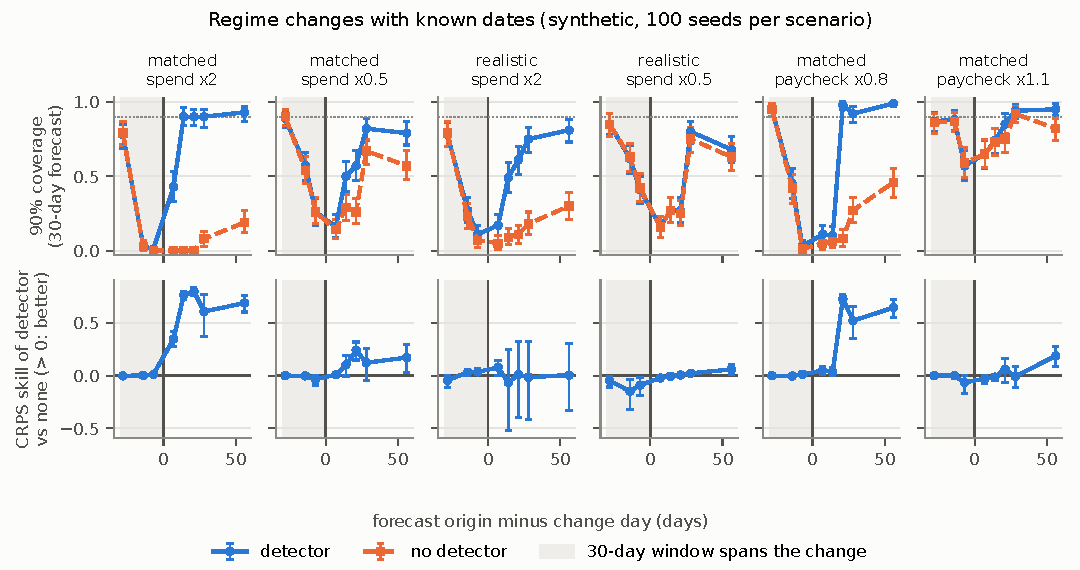
\includegraphics[width=\linewidth]{figures/detector-synthetic.pdf}
\caption{Detector on and off around a known change (synthetic, \hB-day
forecasts, \R{c/ci-level}\% seed-bootstrap intervals). Top: \lC\% coverage.
Bottom: paired CRPS skill of the detector (positive: detector better).
Shaded origins forecast across the change, which no method here can
anticipate.}
\label{fig:detector}
\end{figure}
